% Options for packages loaded elsewhere
% Options for packages loaded elsewhere
\PassOptionsToPackage{unicode}{hyperref}
\PassOptionsToPackage{hyphens}{url}
\PassOptionsToPackage{dvipsnames,svgnames,x11names}{xcolor}
%
\documentclass[
  sn-nature,
]{sn-jnl}


\usepackage{xcolor}
\usepackage{amsmath,amssymb}
\setcounter{secnumdepth}{-\maxdimen} % remove section numbering
\usepackage{iftex}
\ifPDFTeX
  \usepackage[T1]{fontenc}
  \usepackage[utf8]{inputenc}
  \usepackage{textcomp} % provide euro and other symbols
\else % if luatex or xetex
  \usepackage{unicode-math} % this also loads fontspec
  \defaultfontfeatures{Scale=MatchLowercase}
  \defaultfontfeatures[\rmfamily]{Ligatures=TeX,Scale=1}
\fi
\usepackage{lmodern}
\ifPDFTeX\else
  % xetex/luatex font selection
\fi
% Use upquote if available, for straight quotes in verbatim environments
\IfFileExists{upquote.sty}{\usepackage{upquote}}{}
\IfFileExists{microtype.sty}{% use microtype if available
  \usepackage[]{microtype}
  \UseMicrotypeSet[protrusion]{basicmath} % disable protrusion for tt fonts
}{}
\makeatletter
\@ifundefined{KOMAClassName}{% if non-KOMA class
  \IfFileExists{parskip.sty}{%
    \usepackage{parskip}
  }{% else
    \setlength{\parindent}{0pt}
    \setlength{\parskip}{6pt plus 2pt minus 1pt}}
}{% if KOMA class
  \KOMAoptions{parskip=half}}
\makeatother
% Make \paragraph and \subparagraph free-standing
\makeatletter
\ifx\paragraph\undefined\else
  \let\oldparagraph\paragraph
  \renewcommand{\paragraph}{
    \@ifstar
      \xxxParagraphStar
      \xxxParagraphNoStar
  }
  \newcommand{\xxxParagraphStar}[1]{\oldparagraph*{#1}\mbox{}}
  \newcommand{\xxxParagraphNoStar}[1]{\oldparagraph{#1}\mbox{}}
\fi
\ifx\subparagraph\undefined\else
  \let\oldsubparagraph\subparagraph
  \renewcommand{\subparagraph}{
    \@ifstar
      \xxxSubParagraphStar
      \xxxSubParagraphNoStar
  }
  \newcommand{\xxxSubParagraphStar}[1]{\oldsubparagraph*{#1}\mbox{}}
  \newcommand{\xxxSubParagraphNoStar}[1]{\oldsubparagraph{#1}\mbox{}}
\fi
\makeatother


\usepackage{longtable,booktabs,array}
\usepackage{calc} % for calculating minipage widths
% Correct order of tables after \paragraph or \subparagraph
\usepackage{etoolbox}
\makeatletter
\patchcmd\longtable{\par}{\if@noskipsec\mbox{}\fi\par}{}{}
\makeatother
% Allow footnotes in longtable head/foot
\IfFileExists{footnotehyper.sty}{\usepackage{footnotehyper}}{\usepackage{footnote}}
\makesavenoteenv{longtable}
\usepackage{graphicx}
\makeatletter
\newsavebox\pandoc@box
\newcommand*\pandocbounded[1]{% scales image to fit in text height/width
  \sbox\pandoc@box{#1}%
  \Gscale@div\@tempa{\textheight}{\dimexpr\ht\pandoc@box+\dp\pandoc@box\relax}%
  \Gscale@div\@tempb{\linewidth}{\wd\pandoc@box}%
  \ifdim\@tempb\p@<\@tempa\p@\let\@tempa\@tempb\fi% select the smaller of both
  \ifdim\@tempa\p@<\p@\scalebox{\@tempa}{\usebox\pandoc@box}%
  \else\usebox{\pandoc@box}%
  \fi%
}
% Set default figure placement to htbp
\def\fps@figure{htbp}
\makeatother





\setlength{\emergencystretch}{3em} % prevent overfull lines

\providecommand{\tightlist}{%
  \setlength{\itemsep}{0pt}\setlength{\parskip}{0pt}}





%%%% Standard Packages

\usepackage{graphicx}%
\usepackage{multirow}%
\usepackage{amsmath,amssymb,amsfonts}%
\usepackage{amsthm}%
\usepackage{mathrsfs}%
\usepackage[title]{appendix}%
\usepackage{xcolor}%
\usepackage{textcomp}%
\usepackage{manyfoot}%
\usepackage{booktabs}%
\usepackage{algorithm}%
\usepackage{algorithmicx}%
\usepackage{algpseudocode}%
\usepackage{listings}%

%%%%

\raggedbottom
\makeatletter
\@ifpackageloaded{caption}{}{\usepackage{caption}}
\AtBeginDocument{%
\ifdefined\contentsname
  \renewcommand*\contentsname{Table of contents}
\else
  \newcommand\contentsname{Table of contents}
\fi
\ifdefined\listfigurename
  \renewcommand*\listfigurename{List of Figures}
\else
  \newcommand\listfigurename{List of Figures}
\fi
\ifdefined\listtablename
  \renewcommand*\listtablename{List of Tables}
\else
  \newcommand\listtablename{List of Tables}
\fi
\ifdefined\figurename
  \renewcommand*\figurename{Figure}
\else
  \newcommand\figurename{Figure}
\fi
\ifdefined\tablename
  \renewcommand*\tablename{Table}
\else
  \newcommand\tablename{Table}
\fi
}
\@ifpackageloaded{float}{}{\usepackage{float}}
\floatstyle{ruled}
\@ifundefined{c@chapter}{\newfloat{codelisting}{h}{lop}}{\newfloat{codelisting}{h}{lop}[chapter]}
\floatname{codelisting}{Listing}
\newcommand*\listoflistings{\listof{codelisting}{List of Listings}}
\makeatother
\makeatletter
\makeatother
\makeatletter
\@ifpackageloaded{caption}{}{\usepackage{caption}}
\@ifpackageloaded{subcaption}{}{\usepackage{subcaption}}
\makeatother
\usepackage{bookmark}
\IfFileExists{xurl.sty}{\usepackage{xurl}}{} % add URL line breaks if available
\urlstyle{same}
\hypersetup{
  pdftitle={Orchestrating Microbiome Analysis with Bioconductor},
  pdfauthor={Tuomas Borman; Giulio Benedetti; Geraldson Muluh; Aura Raulo; Benjamin Valderrama; Artur Sannikov; Stefanie Peschel; Yihan Liu; Rasmus Hindström; OMA consortium; Katariina Pärnänen; Christian L. Müller; Aki S. Havulinna; Sudarshan Shetty; Marcel Ramos; Domenick J. Braccia; Héctor Corrada Bravo; Felix G.M. Ernst; Levi Waldron; Thomaz F. S. Bastiaanssen; Himel Mallick; Leo Lahti},
  pdfkeywords={microbiome, Bioconductor, data science, data
integration},
  colorlinks=true,
  linkcolor={blue},
  filecolor={Maroon},
  citecolor={Blue},
  urlcolor={Blue},
  pdfcreator={LaTeX via pandoc}}


\title[Orchestrating Microbiome Analysis with
Bioconductor]{Orchestrating Microbiome Analysis with Bioconductor}

% author setup
\author*[1]{\fnm{Tuomas} \sur{Borman}}\email{tuomas.v.borman@utu.fi}\author[1]{\fnm{Giulio} \sur{Benedetti}}\author[1]{\fnm{Geraldson} \sur{Muluh}}\author[3,4]{\fnm{Aura} \sur{Raulo}}\author[5,6]{\fnm{Benjamin} \sur{Valderrama}}\author[2]{\fnm{Artur} \sur{Sannikov}}\author[7]{\fnm{Stefanie} \sur{Peschel}}\author[8,9,10,11,12]{\fnm{Yihan} \sur{Liu}}\author[1]{\fnm{Rasmus} \sur{Hindström}}\author[19]{\fnm{OMA} \sur{consortium}}\author[13]{\fnm{Katariina} \sur{Pärnänen}}\author[7,14,15]{\fnm{Christian L.} \sur{Müller}}\author[1,16]{\fnm{Aki S.} \sur{Havulinna}}\author[17]{\fnm{Sudarshan} \sur{Shetty}}\author[18]{\fnm{Marcel} \sur{Ramos}}\author[19]{\fnm{Domenick J.} \sur{Braccia}}\author[19]{\fnm{Héctor Corrada} \sur{Bravo}}\author[19]{\fnm{Felix G. M.} \sur{Ernst}}\author[18]{\fnm{Levi} \sur{Waldron}}\author[20,21]{\fnm{Thomaz F. S.} \sur{Bastiaanssen}}\equalcont{These authors contributed equally to this work.}\author[8,22,23]{\fnm{Himel} \sur{Mallick}}\equalcont{These authors contributed equally to this work.}\author*[1]{\fnm{Leo} \sur{Lahti}}\email{leo.lahti@utu.fi}
% affil setup
\affil[1]{\orgdiv{Department of Computing}, \orgname{University of
Turku}, \orgaddress{\street{Turku, Finland}}}
\affil[2]{\orgdiv{Department of Life Technologies}, \orgname{University
of Turku}, \orgaddress{\street{Turku, Finland}}}
\affil[3]{\orgdiv{Department of Biology}, \orgname{University of
Oxford}, \orgaddress{\street{Oxford, United Kingdom}}}
\affil[4]{\orgdiv{Queen's College}, \orgname{University of
Oxford}, \orgaddress{\street{Oxford, United Kingdom}}}
\affil[5]{\orgdiv{Department of Anatomy and
Neuroscience}, \orgname{University College
Cork}, \orgaddress{\street{Cork, Ireland}}}
\affil[6]{\orgdiv{APC Microbiome Ireland}, \orgname{University College
Cork}, \orgaddress{\street{Cork, Ireland}}}
\affil[7]{\orgdiv{Department of Statistics}, \orgname{LMU
München}, \orgaddress{\street{Munich, Germany}}}
\affil[8]{\orgdiv{Department of Population Health Sciences, Weill
Cornell Medicine}, \orgname{Cornell University}, \orgaddress{\street{New
York, USA}}}
\affil[9]{\orgdiv{Department of Biomedical Informatics \& Data
Science}, \orgname{Cornell University}, \orgaddress{\street{New York,
USA}}}
\affil[10]{\orgdiv{Department of Biostatistics}, \orgname{Cornell
University}, \orgaddress{\street{New York, USA}}}
\affil[11]{\orgdiv{Department of Biomedical Informatics \& Data
Science}, \orgname{Yale University}, \orgaddress{\street{New Haven,
USA}}}
\affil[12]{\orgdiv{Department of Biostatistics}, \orgname{Yale
University}, \orgaddress{\street{New Haven, USA}}}
\affil[13]{\orgdiv{Department of Microbiology}, \orgname{University of
Helsinki}, \orgaddress{\street{Helsinki, Finland}}}
\affil[14]{, \orgname{Helmholtz Munich}, \orgaddress{\street{Munich,
Germany}}}
\affil[15]{, \orgname{Flatiron Institute}, \orgaddress{\street{New York,
USA}}}
\affil[16]{, \orgname{Institute for Molecular Medicine Finland,
FIMM-HiLIFE}, \orgaddress{\street{Helsinki, Finland}}}
\affil[17]{, \orgname{Danone Research and
Innovation}, \orgaddress{\street{Utrecht, Netherlands}}}
\affil[18]{\orgdiv{Department of Epidemiology and
Biostatistics}, \orgname{CUNY Graduate School of Public Health and
Health Policy}, \orgaddress{\street{New York, USA}}}
\affil[19]{, \orgname{No affiliation}}
\affil[20]{\orgdiv{Department of Psychiatry}, \orgname{Amsterdam
University Medical Centres}, \orgaddress{\street{Amsterdam,
Netherlands}}}
\affil[21]{\orgdiv{Amsterdam Public Health}, \orgname{Amsterdam
University Medical Centres}, \orgaddress{\street{Amsterdam,
Netherlands}}}
\affil[22]{\orgdiv{Division of Gastroenterology and Hepatology, Weill
Cornell Medicine}, \orgname{Cornell University}, \orgaddress{\street{New
York, USA}}}
\affil[23]{\orgdiv{Department of Statistics and Data
Science}, \orgname{Cornell University}, \orgaddress{\street{New York,
USA}}}

% abstract 

\abstract{The expansion of microbiome research has led to the
accumulation of interlinked datasets encompassing versatile taxonomic
and functional assays. The analysis of increasingly large and
heterogeneous multi-modal microbiome data would benefit from unified
approaches supporting the design of modular data science workflows
through interoperable methods. The Bioconductor project recently
developed an optimized statistical programming framework for multi-assay
data integration. Building on this foundation, we introduce a
community-developed, open-source framework for microbiome data science.
In contrast to the previous alternatives, the methodology is
specifically designed to support joint analysis of hierarchical,
interlinked, and heterogeneous multi-table datasets that are
increasingly common in modern microbiome research. This framework
encompasses open data, methods, tutorials, and an active online
community, thereby supporting standardized and reproducible data
wrangling, joint analysis, and reporting. We have detailed the
functionality and usage in the OMA book
(\url{https://bioconductor.org/books/release/OMA}), which offers
guidance for prospective users and contributors.}

% keywords
\keywords{microbiome,  Bioconductor,  data science,  data integration}

\begin{document}
\maketitle


\section{Introduction}\label{sec-intro}

Modern data science applications critically rely on open-source methods
created by the research community \citep{barker2022, pearson2025}. Open
software ecosystems have become central innovation hubs, driving
technological and cultural transformation \citep{hocquet2024}. The
Bioconductor project is a significant distribution channel for open data
science methods in computational life sciences. Its vast developer
community maintains over 2,300 quality-controlled R packages for various
fields of life science informatics \citep{gentleman2004}. Additionally,
Bioconductor has evolved into a global community that supports data
science collaboration and training \citep{drnevich2025}, playing an
increasingly important role in advancing computational skills that are
essential for modern microbiology education \citep{timmis2024}.

Microbiome research focuses on how microbial communities vary, function
and interact with their environment and hosts \citep{moreno-indias2021}.
The technologies used in this field generate vast amounts of
high-dimensional and hierarchically structured data, commonly in the
form of microbial DNA sequences detected in a set of samples. Following
the rapid expansion of microbiome research and technological advances,
metagenomic sequencing is complemented by other types of high-throughput
measurements. This has led to the accumulation of multi-modal
datasets---collections that combine different types of molecular data.
These interlinked datasets encompass diverse taxonomic and functional
assays, ranging from microbial abundances and phylogenetic relationships
to functional profiles. These are summarized into tabular data sets
whose typical sizes range up to tens of thousands of selected features
and samples for downstream statistical analyses.

Microbiome data scientists increasingly face the practical challenges of
integrating heterogeneous and high-dimensional observations across
multiple data modalities into scalable and reproducible workflows
\citep{ragan-kelley2013, callahan2016, holmes2019}. The unique
statistical properties and complexity of microbiome data necessitate
specialized approaches
\citep{moreno-indias2021, jeganathan2021, willis2019, bastiaanssen_bugs1_2023, bastiaanssen_bugs2_2023},
yet the diversity of proposed solutions and inconsistent outcomes
\citep{nearing2022, pelto2025, gamboa-tuz2025} can make it difficult to
identify the optimal methods and build interoperable workflows
\citep{wen2023, shetty2019}. Accordingly, the field can benefit for
standardization and evidence-based best practices
\citep{moreno-indias2021}.

Open microbiome data science \emph{frameworks} have emerged to provide
sets of interoperable methodologies in specific computational
environments \citep{eren2021, schloss2009, bolyen2019, mcmurdie2012},
and a broader ecosystem of digital resources, engaged user communities
and collaboration culture that extend the capacities far beyond the
underlying technical framework. However, frameworks that are focused
solely on microbiome data science fall short on addressing the need to
integrate data across multiple modalities, such as metagenomics,
metabolomics, and host genomics. Bioconductor integrates the methods of
microbiome data science into a wider statistical programming framework,
where interoperable methods for single-cell omics \citep{amezquita2020},
spatial transcriptomics \citep{crowell2025}, metabolomics and proteomics
\citep{anwar2025}, and other fields are concurrently developed.

This approach can introduce some challenges, such as dependency
management, package compatibility, and differences in package stability.
These issues are addressed through coordinated mechanisms that help to
ensure the robustness of the software ecosystem. First, submitted
packages undergo peer review, ensuring relevance and adherence to
standards such as unit tests, reproducible documentation, and working
examples. Secondly, Bioconductor follows a synchronized, semiannual
release cycle, during which packages are frozen and mutually compatible.
Thirdly, all packages are continuously tested within Bioconductor's
automated build system, which ensures that breaking changes are rapidly
detected before release. Each package has an active maintainer who is
notified of failures and responsible for resolving them in a timely
manner. Finally, community guidelines and continuous integration
practices, together with shared data structures such as
(Tree)SummarizedExperiment, further improve interoperability between
packages.

Here, we introduce a stable and optimized data science ecosystem
supporting the integration and analysis of multi-modal datasets in
microbiome research. It provides harmonized data import and
representation, and fast, robust methods for transforming abundance
tables into biological insights. These methods have been extensively
tested and distributed through mature R/Bioconductor packages
(\url{https://bioconductor.org/packages}), supporting the
community-driven development and integration within the broader
Bioconductor ecosystem. To promote evidence-based best practices, we
introduce the online book \emph{Orchestrating Microbiome Analysis with
Bioconductor} (OMA), which represents a comprehensive compilation of
established approaches and emerging trends in microbiome data science
using the R/Bioconductor ecosystem.

\section{Data infrastructure}\label{sec-infra}

Data scientists routinely deal with interlinked assays, hierarchical
data (\emph{e.g.}, ontologies, trees), relational data (\emph{e.g.},
networks), and supporting side information. This side information can
include sample attributes such as treatment group, collection site, or
time point. The ability to integrate heterogeneous data elements is
essential in biological research, where the individual components of a
system can seldom be studied in isolation. However, this growing
complexity introduces additional overhead, as researchers must track
samples and features across multiple tables and manage an increasing
number of data elements and non-trivial links between them. Moreover,
input data formats vary across methods, leading to technical
complications and time lost on data wrangling. Bioconductor addresses
these challenges through standardized data structures that are extended
by an ecosystem of quality-controlled, interoperable methods. Adopting
the framework will thus allow the analyst to avoid unnecessary data
wrangling and invest more time in core analytical tasks.

Bioconductor data structures support statistical analysis of complex
data combinations \citep{huber2015} and are widely adopted in omics
research (Figure~\ref{fig-bioc_packages}). They have been implemented
through specialized object-oriented classes that integrate multiple data
elements into a single structure known as a \emph{data container}. The
SummarizedExperiment (SE) class \citep{huber2015} is the primary data
container underlying the Bioconductor ecosystem (Figure
\ref{fig:datacontainers}a and Table~\ref{tbl-elements}). Its position
among the top 1\% most-downloaded packages in Bioconductor reflects its
widespread recognition and increasing adoption among developers. It
provides a standardized solution to store tabular data by linking
numeric abundance matrices with rich side information on the
features/rows (\emph{e.g.}, taxonomy), and samples/columns (\emph{e.g.},
origin, collection time, host health).

The vast adoption and interoperability of SE-based data structures
enables the transfer of methods across different fields of omics
research, thereby promoting the development of modular and scalable data
science methods and yielding improved overall quality control and user
support \citep{drnevich2025}. The SE framework has been extended to
similar data integration tasks, notably in single-cell and spatial omics
through the SingleCellExperiment (SCE) \citep{amezquita2020} and
SpatialExperiment \citep{righelli2022} classes.

\begin{figure}

\centering{

\pandocbounded{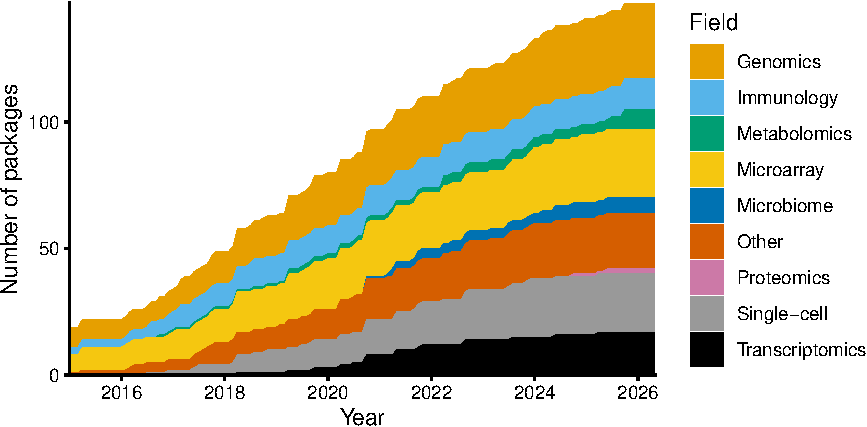
\includegraphics[keepaspectratio]{manuscript_files/figure-pdf/fig-bioc_packages-1.pdf}}

}

\caption{\label{fig-bioc_packages}\textbf{Adoption of the
SummarizedExperiment (SE) data container among Bioconductor developers.}
The growth in the number of Bioconductor packages supporting SE over
time is shown, categorized by their respective fields. Packages are
counted by the date they were added to Bioconductor. Some packages added
the SE support after their original release.}

\end{figure}%

\textbf{Hierarchical data structures.} Microbiome data scientists
frequently need to integrate information on feature phylogenies and
sample hierarchies to accurately reflect fine-scale variability in
microbiome data. While maintaining interoperability with the broader
Bioconductor ecosystem, the TreeSummarizedExperiment (TreeSE) class
\citep{huang2021} extends the SE and SCE data structures to hierarchical
datasets by incorporating both feature and sample organizations as tree
structures (Figure \ref{fig:datacontainers}b and
Table~\ref{tbl-elements}). Beyond the core components of microbiome
datasets, including taxa abundances, sample metadata, phylogenetic
trees, and reference sequences, TreeSE provides a flexible foundation
for multi-modal data integration, supporting the incorporation of
functional predictions, resistome, metabolome, and other molecular
profiles, as well as alternative feature representations. It can also
store results from common analytical procedures, such as statistical
transformations or agglomeration. By inheriting full compatibility with
SE and SCE, TreeSE enables the development of modular, interoperable
workflows across the Bioconductor ecosystem.

\begin{center}
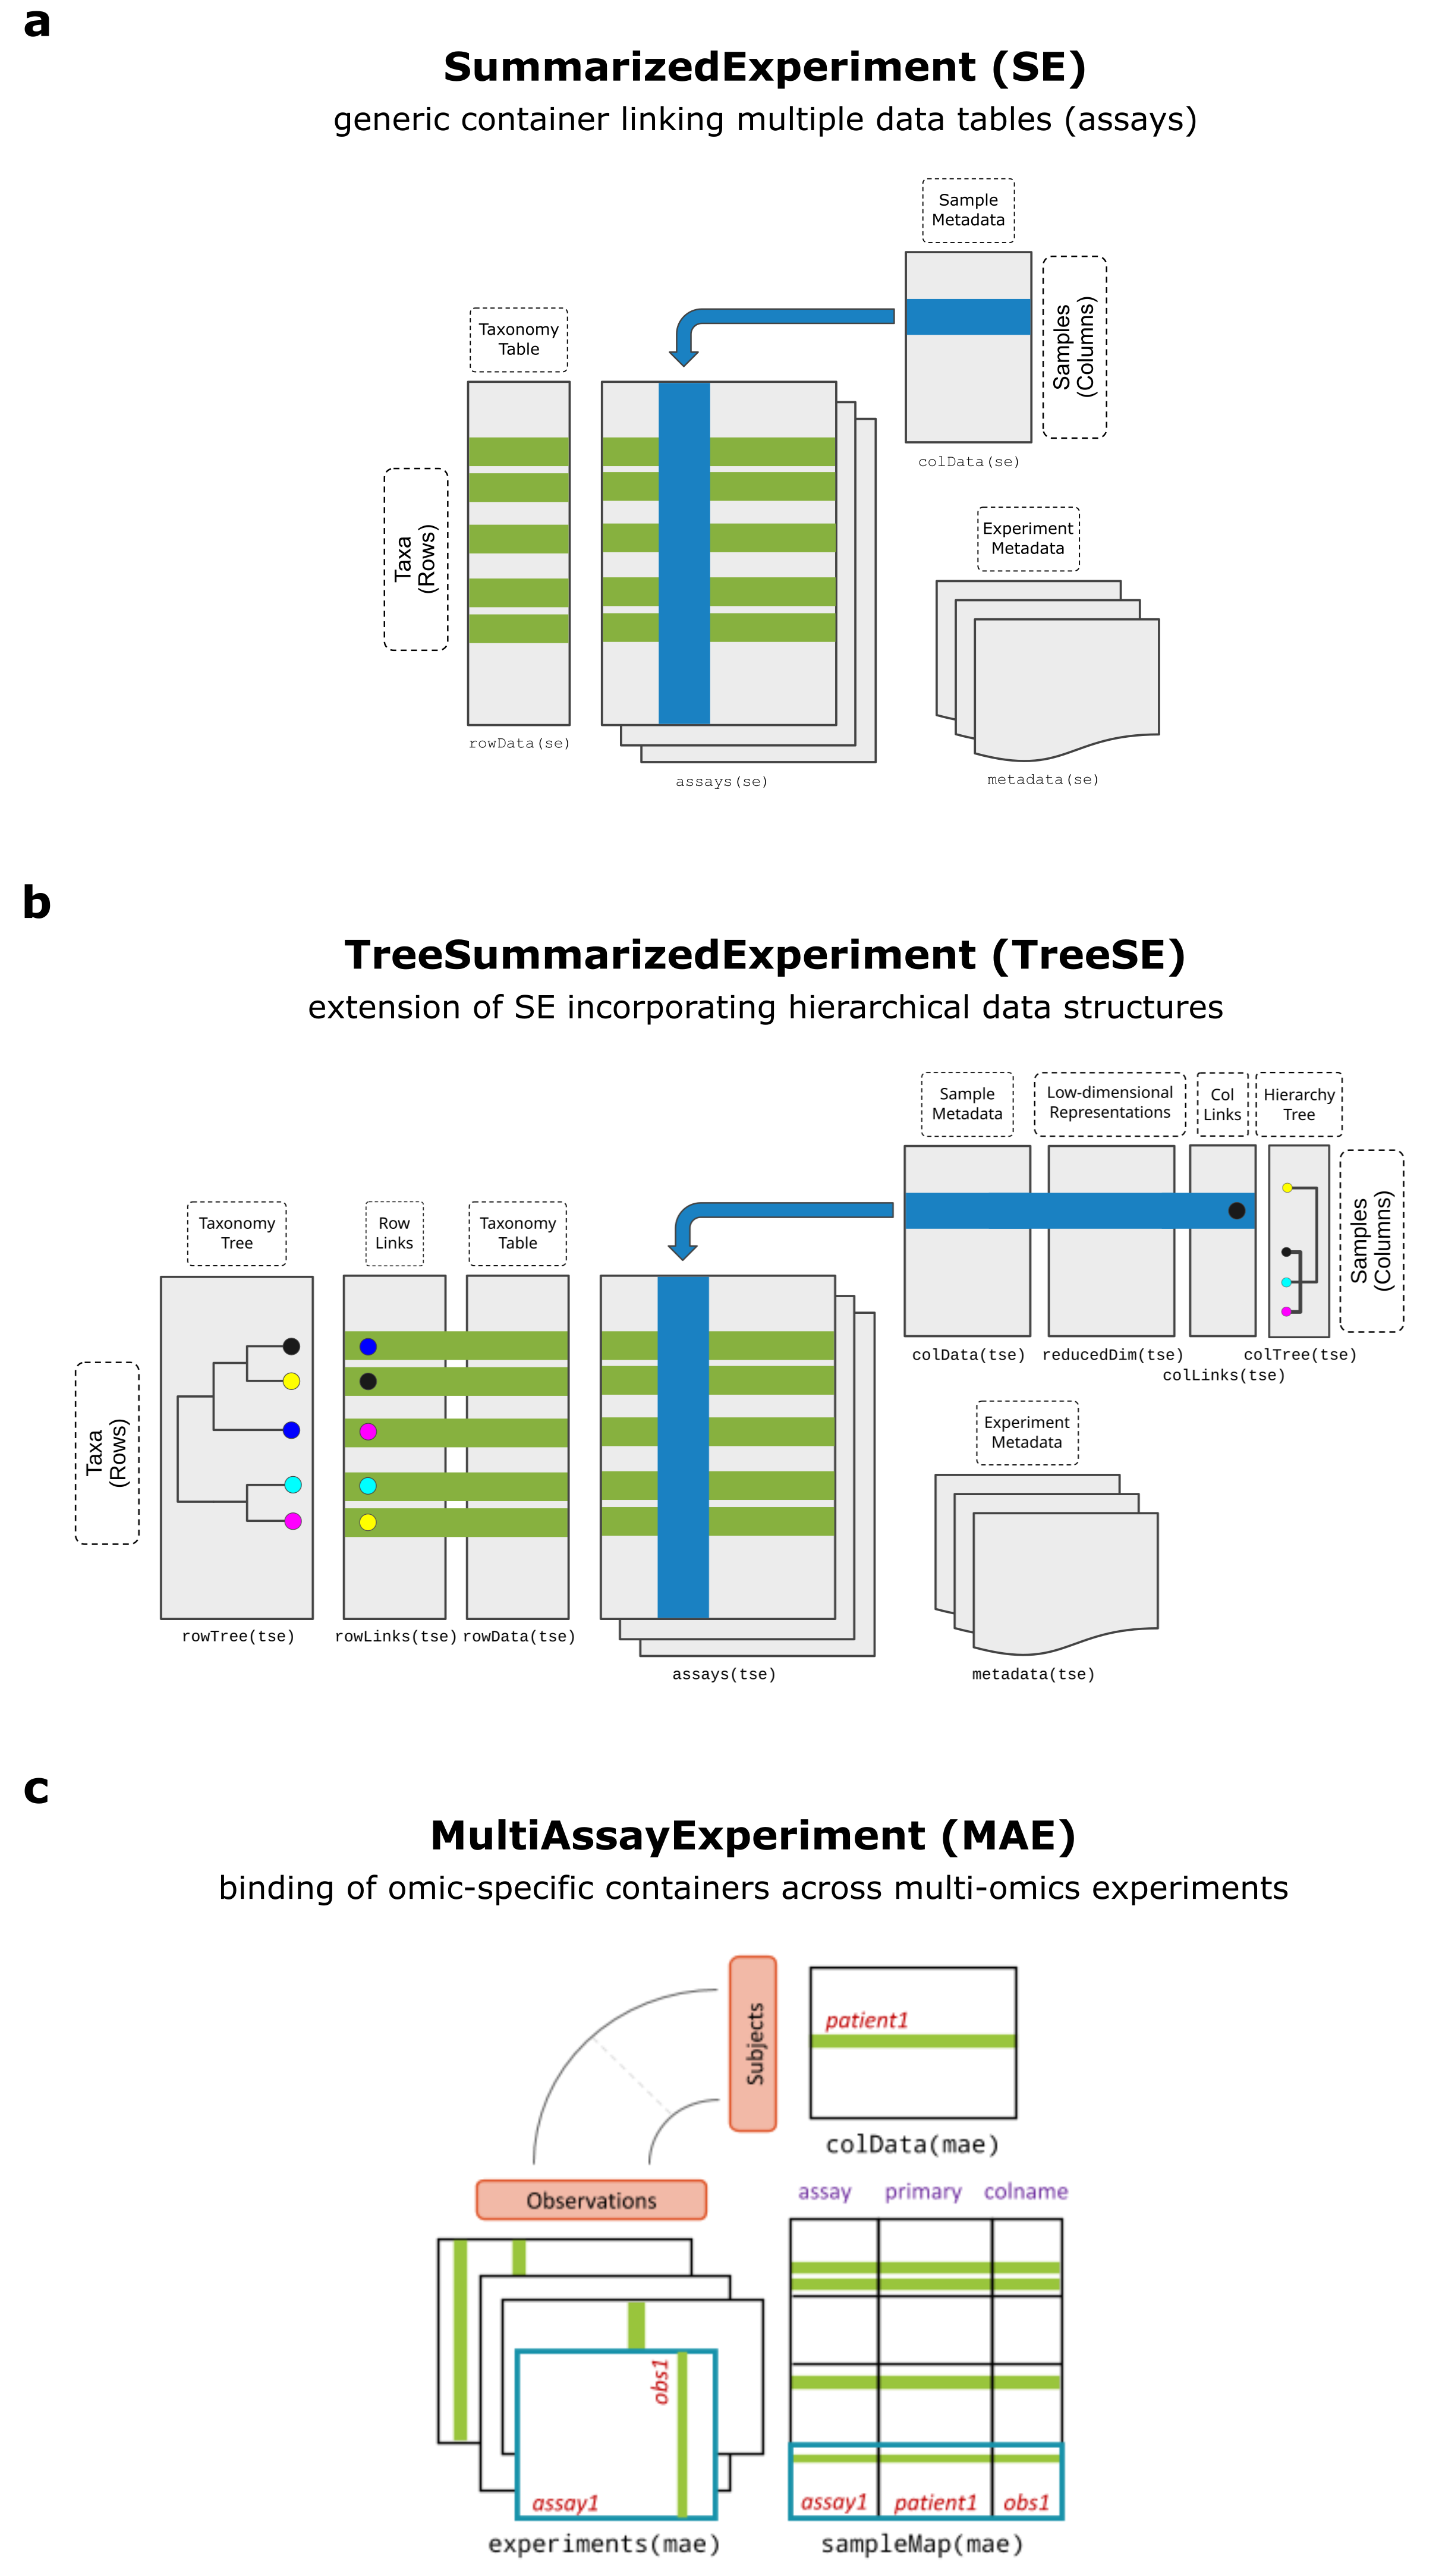
\includegraphics[height=\textheight]{figures/data_containers.png}
\end{center}
\captionof{figure}{\textbf{Integrative Bioconductor containers for microbiome data.}
\textbf{(a) SummarizedExperiment (SE)} \cite{huber2015} is a generic container
for single-omics experiments. It accommodates \textit{assays} that describe the
feature abundances in each sample (\textit{e.g.}, taxonomic units, resistance
genes, or predicted functions), and tabular side information on each sample
(\textit{colData}) and feature (\textit{rowData}), \textit{e.g.}, the taxonomic
classification.
\textbf{(b) TreeSummarizedExperiment (TreeSE)} \cite{huang2021} supports
hierarchical, multi-table microbiome analysis. In addition to the SE elements,
TreeSE incorporates tree information on feature hierarchies, such as
phylogenetic relations between the taxonomic units (\textit{rowTree}) or host
species (\textit{colTree}), and results of dimensionality reduction
(\textit{reducedDims}). TreeSE can thus link multiple abundance tables
and their transformed versions (\textit{e.g.}, statistical transformation,
taxonomic agglomeration, or dimensionality reduction) with tabular and
hierarchical side information on the features (rows) and samples (columns).
Additional slots for reference sequences and experiment metadata are available.
\textbf{(c) MultiAssayExperiment (MAE)} \cite{ramos2017} facilitates the
integration of interlinked datasets representing different omics modalities
linked by potentially non-trivial sample mappings. Figure adapted from \cite{ramos2017}.}

\label{fig:datacontainers}

\textbf{Multi-assay data structures.} Contemporary microbiome research
frequently involves data across multiple measurement modalities for
enhanced functional and mechanistic insights. This brings the need to
find an appropriate representation for each data type and map the links
between them. Whereas the TreeSE data container is broadly applicable to
different modalities such as taxonomic, resistome, transcriptome,
proteome, and metabolome profiling data, dedicated data containers have
been developed for certain modalities by the Bioconductor community to
address their specific characteristics; examples include single-cell
sequencing \citep{amezquita2020} and host genomics \citep{lawrence2013}.
Linking data across modalities presents an additional technical
challenge, as multi-omics datasets are often sparse so that only a
subset of the samples may be shared across multiple modalities
\citep{sherwani2025}. In other cases, a single sample in one modality
may link to several samples in another modality \citep{husso2023}
(\emph{e.g.}, due to technical or spatial replication). These scenarios
require the ability to integrate multiple data modalities into a single
object and create flexible sample mappings across them. The
MultiAssayExperiment (MAE) data container \citep{ramos2017} addresses
these challenges by introducing a formal mapping layer (sampleMap) that
links biological samples to their corresponding measurements in each
modality (Figure \ref{fig:datacontainers}c and
Table~\ref{tbl-elements}). This design supports one-to-one, one-to-many,
and partially overlapping sample relationships across experiments.
Importantly, this mapping is also accessible for downstream operations.
For instance, when subsetting a MAE object (\emph{e.g.}, selecting
samples with both microbiome and metabolome data), the framework
automatically resolves the intersection of available samples and ensures
consistent alignment across all modalities. Such structured handling of
sample relationships is particularly important for integrative methods,
as it reduces the risk of sample mismatches, a common source of
irreproducibility in ad hoc multi-table analyses. To summarize, flexible
mapping of samples across several data objects is a key for efficient
data integration, method sharing, and interoperability.

\textbf{Scalability} Enhanced scalability is one of the advantages of
our framework, and essential with increasingly large and multi-modal
data sets. This can be achieved by parallelization, out-of-memory
analyses leveraging the built-in support for sparse and delayed
matrices, more efficient implementations through code optimization,
executing costly computations in C++, and methodological advancements.
In many cases, the support can be readily inherited from the underlying
Bioconductor infrastructure, rather than newly implemented
\citep{lun2018beachmat}. For instance, the (Tree)SE and MAE containers
are agnostic to assay representation and natively support sparse
(dgCMatrix, SparseArray) and file-backed (HDF5Array, DelayedArray)
assays \citep{huber2015}. Many methods readily support parallelization;
BiocParallel can support operations that decompose into independent
blocks by samples, features, or other data elements. Non-decomposable
operations, such as distance matrices and ordinations, must be realized
in memory or parallelized by a dedicated algorithm: accelerated versions
of common microbiome methods, including Faith phylogenetic alpha
diversity \citep{armstrong2021} and striped Unifrac beta diversity
\citep{mcdonald2018}, have been incorporated in the (Tree)SE-based
framework through the mia package.

\begin{longtable}[]{@{}
  >{\raggedright\arraybackslash}p{(\linewidth - 8\tabcolsep) * \real{0.1800}}
  >{\raggedright\arraybackslash}p{(\linewidth - 8\tabcolsep) * \real{0.6200}}
  >{\centering\arraybackslash}p{(\linewidth - 8\tabcolsep) * \real{0.0300}}
  >{\centering\arraybackslash}p{(\linewidth - 8\tabcolsep) * \real{0.0900}}
  >{\centering\arraybackslash}p{(\linewidth - 8\tabcolsep) * \real{0.0800}}@{}}
\caption{Key elements of the Bioconductor data containers for microbiome
analysis. }\label{tbl-elements}\tabularnewline
\toprule\noalign{}
\begin{minipage}[b]{\linewidth}\raggedright
Slot
\end{minipage} & \begin{minipage}[b]{\linewidth}\raggedright
Content
\end{minipage} & \begin{minipage}[b]{\linewidth}\centering
SE
\end{minipage} & \begin{minipage}[b]{\linewidth}\centering
TreeSE
\end{minipage} & \begin{minipage}[b]{\linewidth}\centering
MAE\(^a\)
\end{minipage} \\
\midrule\noalign{}
\endfirsthead
\toprule\noalign{}
\begin{minipage}[b]{\linewidth}\raggedright
Slot
\end{minipage} & \begin{minipage}[b]{\linewidth}\raggedright
Content
\end{minipage} & \begin{minipage}[b]{\linewidth}\centering
SE
\end{minipage} & \begin{minipage}[b]{\linewidth}\centering
TreeSE
\end{minipage} & \begin{minipage}[b]{\linewidth}\centering
MAE\(^a\)
\end{minipage} \\
\midrule\noalign{}
\endhead
\bottomrule\noalign{}
\endlastfoot
\textbf{Tables} & & & & \\
assays & tables of features (rows) and samples (cols) & X & X & X \\
altExps\(^b\) & experiments with variable number of features & & X &
X \\
reducedDims & results of dimensionality reduction & & X & X \\
\textbf{Rows} & & & & \\
rowData & side information on features & X & X & X \\
rowPairs & linkage between pairs of associated features & & X & X \\
rowTrees & hierarchical organization of features & & X & X \\
referenceSeq & reference sequences of features & & X & X \\
\textbf{Columns} & & & & \\
colData & side information on samples & X & X & X \\
colTrees & hierarchical organization of samples & & X & X \\
sampleMap\(^c\) & flexible sample mapping across experiments & & & X \\
\textbf{Other} & & & & \\
metadata & additional information on the experiment & X & X & X \\
\end{longtable}

\(^a\)While MAE does not contain conventional slots (with the exception
of colData), its experiments can include any number of data containers
that provide those slots. \(^b\)altExp samples must match assay samples
in a 1-to-1 mapping. \(^c\)The sampleMap supports diverse mappings
between samples from different experiments (1-to-1, 1-to-many, many-to-1
and many-to-many). SE, SummarizedExperiment; TreeSE,
TreeSummarizedExperiment; MAE, MultiAssayExperiment.

\textbf{Data resources.} Several open microbiome data resources are
supported by this framework, enabling direct data import into the
aforementioned data containers for further downstream analysis within
R/Bioconductor (Table~\ref{tbl-dataresources}). Examples include
curatedMetagenomicData \citep{pasolli2017}, HoloFood \citep{rogers2024},
microbiomeDataSets (Bioconductor package), and the EBI/MGnify database
\citep{gurbich2023}. Bioconductor packages include additional built-in
demonstration datasets. Collectively, these resources encompass
taxonomic and functional profiles from thousands of published microbiome
studies and tens of thousands samples that can be accessed with the
available tools for research and educational purposes.

\begin{longtable}[]{@{}
  >{\raggedright\arraybackslash}p{(\linewidth - 6\tabcolsep) * \real{0.4000}}
  >{\centering\arraybackslash}p{(\linewidth - 6\tabcolsep) * \real{0.2000}}
  >{\raggedleft\arraybackslash}p{(\linewidth - 6\tabcolsep) * \real{0.2000}}
  >{\raggedleft\arraybackslash}p{(\linewidth - 6\tabcolsep) * \real{0.2000}}@{}}
\caption{Open microbiome data resources (last accessed on 2026-07-05).
}\label{tbl-dataresources}\tabularnewline
\toprule\noalign{}
\begin{minipage}[b]{\linewidth}\raggedright
Data resource / Package
\end{minipage} & \begin{minipage}[b]{\linewidth}\centering
References
\end{minipage} & \begin{minipage}[b]{\linewidth}\raggedleft
\# Studies
\end{minipage} & \begin{minipage}[b]{\linewidth}\raggedleft
\# Samples
\end{minipage} \\
\midrule\noalign{}
\endfirsthead
\toprule\noalign{}
\begin{minipage}[b]{\linewidth}\raggedright
Data resource / Package
\end{minipage} & \begin{minipage}[b]{\linewidth}\centering
References
\end{minipage} & \begin{minipage}[b]{\linewidth}\raggedleft
\# Studies
\end{minipage} & \begin{minipage}[b]{\linewidth}\raggedleft
\# Samples
\end{minipage} \\
\midrule\noalign{}
\endhead
\bottomrule\noalign{}
\endlastfoot
MGnifyR\(^a\) & \citep{gurbich2023} & 5,616 & 429,108 \\
Metalog\(^b\) & \citep{kuhn2026} & 1,074 & 157,483 \\
curatedMetagenomicData\(^a\) & \citep{pasolli2017} & 93 & 22,588 \\
miaData\(^c\) & & 9 & 20,404 \\
microbiomeDataSets\(^a\) & & 6 & 19,100 \\
HMP2data\(^a\) & & 3 & 11,493 \\
HoloFoodR\(^{a,d}\) & \citep{rogers2024, borman2025} & 9 & 9,990 \\
MicrobiomeBenchmarkData\(^a\) & \citep{gamboa-tuz2025} & 6 & 1,125 \\
\end{longtable}

\(^a\)Bioconductor package with the corresponding name. \(^b\)Data
retrieval to TreeSE format instructed in OMA online book. \(^c\)Zenodo
mia community. \(^d\)HoloFood microbiome datasets are deposited in the
MGnify database. HMP, Human Microbiome Project.

\section{Alternative frameworks}\label{sec-data_frameworks}

Several alternative frameworks to microbiome analysis are available.
Within Bioconductor, phyloseq \citep{mcmurdie2012} provides widely
adopted tools with a primary focus on 16S amplicon data analysis.
(Tree)SE accommodates all core components of phyloseq objects, including
abundance tables, taxonomic annotations, phylogenetic trees, reference
sequences, and sample metadata. The advantages of newer (Tree)SE
container \citep{huber2015} include many additional data elements, a
better integration with the overall Bioconductor ecosystem, and enhanced
support for multi-assay analyses (see \hyperref[sec-infra]{Data
infrastructure}). Thus, some originally phyloseq-based tools, such as
microbiome R/Bioconductor package \citep{shetty2019}, have been recently
extended with TreeSE support.

Related frameworks beyond R/Bioconductor include command-line toolkits
supported by active user and developer communities. Mothur
\citep{schloss2009} is primarily designed for 16S amplicon analysis and
less well suited for integrative metagenomics and multi-omics. QIIME 2
\citep{bolyen2019} is a Python-based, AI-ready microbiome multi-omics
data science platform. It primarily targets amplicon and metagenomic
analyses, and incorporates methods from scikit-bio Python library
\citep{aton2026} which supports multi-omic integration tasks. A
particular advantage of these frameworks is their direct connection with
the strong machine learning and AI ecosystem in Python, while the
interoperability with independently developed omics tools may remain
more limited. Anvi'o \citep{eren2021} is a complementary,
community-driven analysis and visualization platform for microbial
'omics with a distinct focus on genome-resolved metagenomics and
detailed sequence-level analyses. These frameworks emphasize
standardized, modular approaches tailored to microbiome analysis and
provide validated and user-friendly solutions, supporting efficient
end-to-end workflows for microbiome research. Bioconductor emphasizes
broad interoperability and shared statistical programming infrastructure
with other areas of omics research, and primarily serves the R
community. To facilitate migration from alternative frameworks, the OMA
book provides conversion tables and utility functions to convert between
TreeSE and many external data formats.

Quantitative comparisons indicate enhanced scalability over commonly
used alternatives (Figure~\ref{fig-benchmarking} and Supplementary
Figure 1). We executed routine operations on increasingly large subsets
of the Metalog database \citep{kuhn2026}, and measured the execution
time and memory consumption with TreeSE, phyloseq, speedyseq, and QIIME
2. Overall, (Tree)SE scaled most efficiently in execution time and
memory allocation with increasing feature and sample sizes. It is
applicable to abundance matrices of up to 100,000 samples and 10,000
features on a standard laptop, except for the heaviest operations such
as phylogenetic beta diversity (UniFrac) calculation, where the general
break point is reached around 10,000 samples with all methods. At a
feature set size of 10,000 the break point is additionally reached with
the PhILR transformation and melting operation. At smaller sample sizes
phyloseq or its accelerated extension speedyseq are occasionally faster
but these differences are moderate (few seconds on a standard laptop).
QIIME 2 is generally slower on lower sample sizes but scales well with
increasing sample sizes. Despite the advantages, optimizing time and
memory consumption represents a key area for further development.

\begin{figure}

\centering{

\pandocbounded{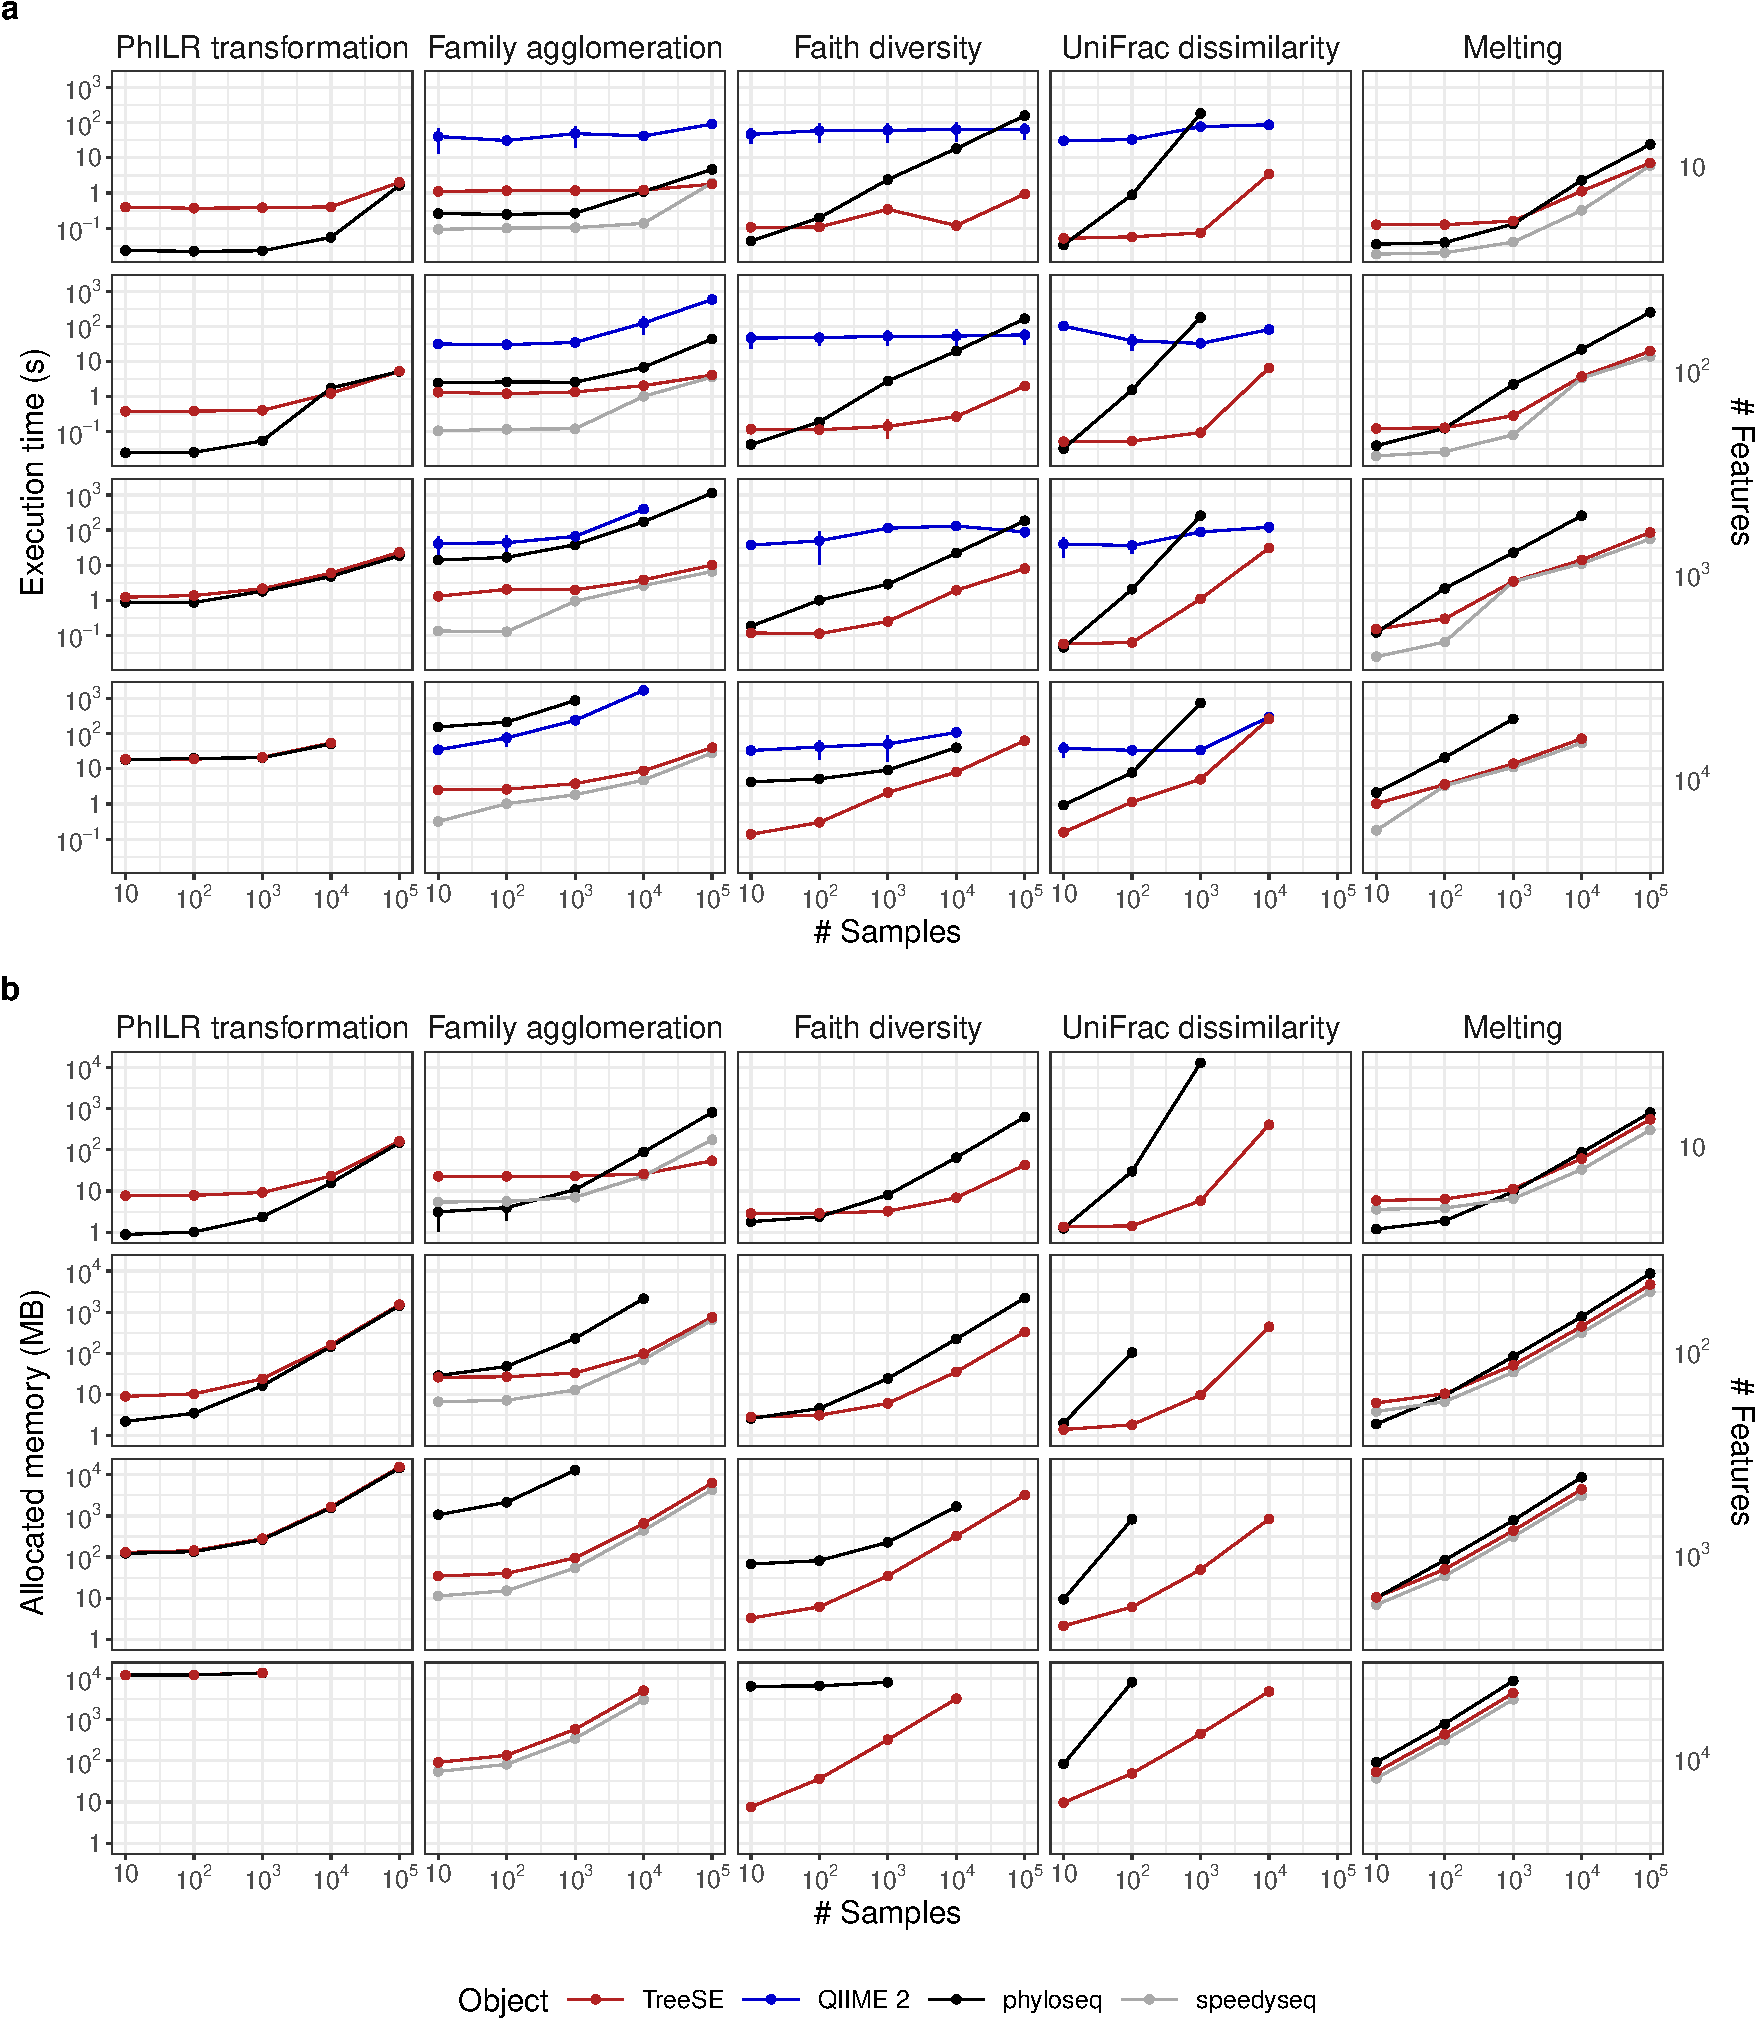
\includegraphics[keepaspectratio]{manuscript_files/figure-pdf/fig-benchmarking-1.pdf}}

}

\caption{\label{fig-benchmarking}\textbf{Execution time and allocated
memory for routine microbiome data operations.}
TreeSummarizedExperiment, QIIME 2 and phyloseq---with its extension
speedyseq---are three popular frameworks for microbiome analysis. We
benchmarked them for five routine operations applied to random subsets
of features (rows) and samples (columns) from the Metalog database
\citep{kuhn2026}. Both execution time (s) and allocated memory (MB) were
measured as the mean value over ten replicates with varying subsets of
the same dimension. Errorbars show the 95\% confidence interval of the
performance estimate. The benchmarking was conducted in R using the
bench library with 4 CPU cores and 16 GB RAM. QIIME 2 lacks allocated
memory estimates because memory cannot be monitored for external
processes. The source code for the benchmarking analysis is openly
available in the Zenodo mia community.}

\end{figure}%

\section{Data preparation}\label{sec-process}

While several tools for microbiome data analysis are available
\citep{jeganathan2021, willis2019, marcoszambrano2023}, their
implementations typically differ in terms of expected input and output
formats. Common data standards promote modular workflows, speeding up
methods development, benchmarking, and replication. Building upon these
principles, we describe a set of interoperable software libraries that
support microbiome data integration and analysis based on the two
integrative data containers, TreeSE and MAE (Figure \ref{fig:workflow}).

This framework specifically supports the downstream analysis of
high-throughput sequencing data from microbiome experiments, after
summarizing the original measurements into abundance tables
(\emph{e.g.}, taxonomic or functional profiles). Taxonomic abundance
tables are one of the most commonly encountered data types in
contemporary microbiome studies. Common measurement platforms include
amplicon-based marker gene studies (\emph{e.g.}, 16S rRNA) and
metagenomic sequencing, processed with methods such as MetaPhlAn
\citep{blanco2023} or Greengenes2 \citep{mcDonald2024Greengenes2}.
Alternative profiling techniques are available, including phylogenetic
microarrays \citep{rajilicstojanovic2009} and high-density optical
mapping \citep{abakumov2024}. Tabular abundance data can also arise from
resistome profiling, mapping of other genomic elements, or from
functional measurements. The framework is agnostic to the source of
abundance data but many of our methodological choices have been guided
by data tables that are typical for microbiome profiling studies.

\textbf{Data import.} While the TreeSE data container can be populated
with microbiome data from common tabular data types, non-standard file
formats may require additional data wrangling. To streamline data
import, we provide importers for a variety of standard microbiome file
formats, including BIOM \citep{mcdonald2012}, MetaPhlAn/HUMAnN (versions
2-4) \citep{beghini2021}, Mothur \citep{schloss2009}, QIIME 2
\citep{bolyen2019}, and the TAXonomic Profile Aggregation and
standardization format (taxpasta) \citep{beber2023}. External to
Bioconductor, the qiime2R package provides additional functionality to
create TreeSE objects directly from QIIME 2 artifacts.

These importers retain provenance of the metadata and the conversion
workflow, bridging the gap between the original data processing, other
tools, and downstream statistical analysis in R. This allows researchers
to focus on interpreting biological patterns rather than wrangling file
formats. Moreover, converters between alternative data structures in R
are available supporting seamless conversions between TreeSE and BIOM,
DADA2 \citep{callahan2016}, and phyloseq (the mia::convert* functions).
Imported datasets from different omics modalities can then be
interlinked within the MAE data container with its flexible sample
mappings as described above. This integrated data object can then be
analyzed with dedicated downstream methods.

Similarly, microbiome data stored in TreeSE objects can be exported to
external services such as MicrobiomeDB \citep{oliveira2018} and to other
languages (\emph{e.g.}, Julia). These converters facilitate widespread
access to microbiome analysis methods.

\textbf{Quality control and exploration.} After importing the data into
R, the recommended first step involves basic data exploration and
quality control \citep{zuur2010}. In addition to methods for identifying
contaminant sequences and calculating summary statistics, the framework
includes a versatile set of custom visualization methods to assess data
variability, outliers, homogeneity of variance and other aspects that
may need to be considered in downstream data analysis. The mia and
miaViz packages provide convenient access to many operations for the
integrative data containers regarding common tasks in microbiome data
exploration and visualization (\textbf{?@fig-downstream\_analyses}).

\textbf{Filtering and agglomeration.} Microbiome datasets can contain
tens of thousands of unique features depending on the sequencing
resolution, used reference databases, and the scope of analysis.
Moreover, the integration of multiple omics modalities adds another
level of challenges. To summarize data into biologically meaningful
groups or to reduce multiple comparisons the data is often subsetted,
filtered or agglomerated to higher-level taxonomic or functional
categories or stratified by sample groups. The package ecosystem, and
the mia package in particular, feature various tools for such tasks. For
instance, the prevalence-based methods can be helpful to remove rare
features that are likely sequencing artifacts or present otherwise
limited value for the analysis. The mechanism of alternative experiments
(altExp) allows agglomeration by taxonomic levels or other features such
as pathogenicity or functional potential (\emph{e.g.}, butyrate
production \citep{kullberg2024}, gut-brain modules
\citep{vallescolomer2019}, and host-associated signatures as in the
BugSigDB \citep{geistlinger2024}). The agglomerated data can be
incorporated as a new alternative experiment within the original data
object. The automated tracking of feature and sample links ensures that
changes are propagated across all relevant elements of the data object,
such as transformed abundance tables, phylogenetic trees, or interlinked
omics modalities. This helps to avoid redundant processing and enables
efficient management of interlinked datasets.

\textbf{Transformation.} Statistical transformations commonly used in
microbiome research include relative abundance \citep{gloor2017},
phylogenetic ILR (PhILR) \citep{silverman2017}, centered log-ratio
(CLR), and robust CLR (rCLR) \citep{martino2019}. The latter three aim
to mitigate compositionality bias. A related concept that controls for
unequal sampling depth is data rarefaction, i.e.~repeatedly subsampling
data to equal read depth and averaging the computed metrics to mitigate
information loss \citep{schloss2024b} that could arise from subsampling
(\emph{rarefying}) data to equal read depth without such iteration
\citep{mcmurdie2014, schloss2024, willis2019b}. Our framework supports
these and a variety of other transformations commonly applied to
microbiome data.

\textbf{Data enrichment.} Incorporating additional data, such as
transformed feature abundance tables, is a frequent operation in applied
data analysis, and it often takes place iteratively. The integrative
data containers support gradual and organized accumulation of
interlinked data elements including alpha and beta diversity, prevalence
calculations, transformations, agglomerated data, reduced dimensions,
and other derived data on samples and features. We generally recommend
initializing the data objects by pre-calculating such measures already
at the beginning of the workflow, where they can then be gradually
enriched as the project advances. By systematically extending the
upstream data preparation step, instead of ad-hoc calculations scattered
amidst the workflow, one can achieve a well-organized and transparent
provenance of the integrated data object.

\begin{center}
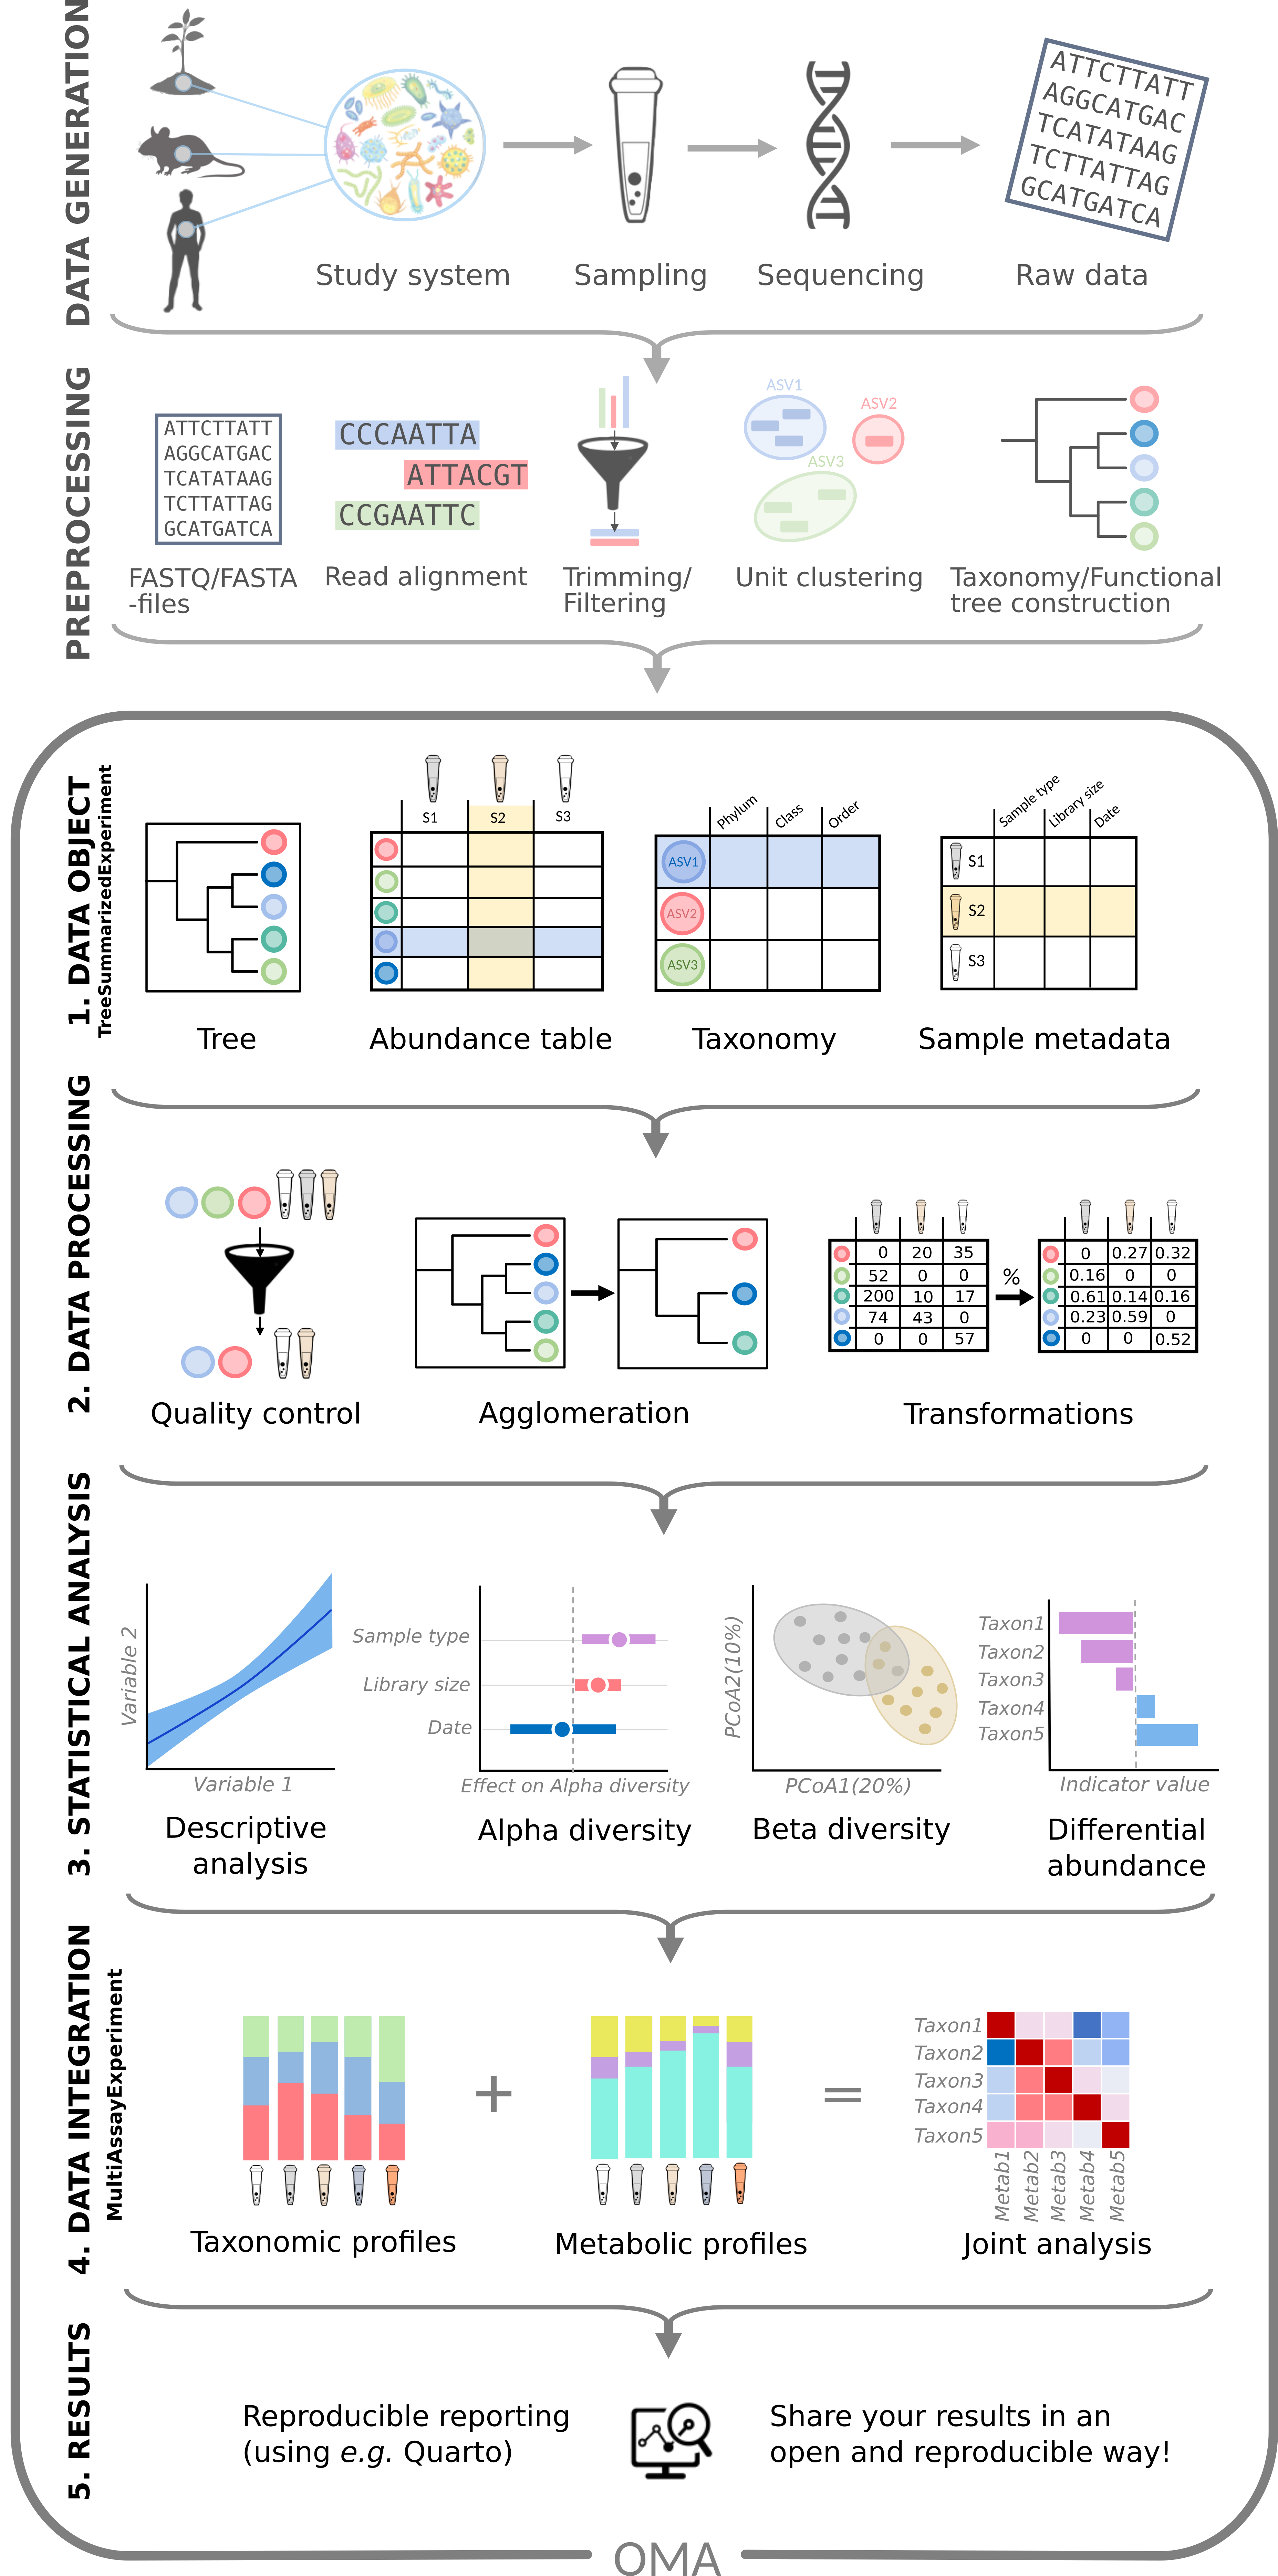
\includegraphics[height=\textheight]{figures/workflow.png}
\end{center}
\captionof{figure}{\textbf{Multi-modal data integration workflow.} Following
data generation and preprocessing (top two panels), the integrative framework
covers five steps of microbiome data integration and analysis: 1) Data is
combined into a TreeSummarizedExperiment (TreeSE) data container,
storing information on the samples (tube icons) and their features
(\textit{e.g.}, taxonomic, functional, or resistome profiles; colored circles).
TreeSE objects can accommodate multiple assay tables as well as additional
hierarchical structures. 2) The TreeSE data object can then be processed to clean
the data. This involves filtering out low-quality samples and features,
transforming assays for example by normalizing feature-wise to enhance the
comparability of sample-specific abundances, or agglomerating features
to specific taxonomic levels or functional categories. 3) The cleaned data can
then be analyzed using statistical models to uncover relations among samples
(\textit{e.g.}, with ordination methods), analyze drivers of variation in community diversity
and composition, or test for differential abundance (\textit{e.g.} between
sampling time or location). 4) The framework supports the integration of
various types of omics modalities through the MultiAssayExperiment and
omic-specific data containers provided by Bioconductor.
For example, the taxonomic and metabolomic profiles of samples can be summarized
and compared in a joint analysis among features. 5) Finally, Quarto notebooks
aid reproducible analysis and reporting.}

\label{fig:workflow}

\section{Downstream data analysis}\label{sec-analysis}

Our framework has been designed to improve the management of integrative
multi-omic workflows. It facilitates joint operations on interlinked
data elements, helping to shift the focus towards multi-modal analyses
and methods development while also supporting standard data analyses in
microbiome research.

Microbiome data analysis often relies on specialized statistical
approaches, since data sparsity, zero-inflation, compositionality, and
heteroscedasticity pose challenges for standard methods
\citep{gloor2017, jeganathan2021}. Furthermore, microbiome data is
hierarchically structured across taxonomic, ecological, temporal, and
spatial levels \citep{moreno-indias2021, sherwani2025, ruuskanen2021}.
Alternative processing pipelines introduce different biases and generate
varying data formats; for example, the same sample can yield differing
taxonomic profiles depending on the computational method used
\citep{quince2017}. These and other unique characteristics have
wide-reaching implications for microbiome analysis, necessitating
dedicated analysis methods \citep{moreno-indias2021, jeganathan2021}.
The shared data containers support community-driven development and
reproducible benchmarking.

The following sections provide an overview of some of the currently
available tools, encompassing standard methods for taxonomic,
metagenomic, and functional abundance tables as well as integrative
analyses between modalities.

\textbf{Community indicators.} Various general indicators are available
to quantify the microbial community state or other sample properties.
Community diversity is a common measure in microbial ecology
\citep{bastiaanssen_bugs1_2023} (\textbf{?@fig-downstream\_analyses}).
Alpha diversity metrics generally quantify the observed or estimated
number of distinct taxa (\emph{richness}) and their distribution
(\emph{evenness}). Many diversity indices (\emph{e.g.}, Shannon index),
combine these two aspects. Phylogenetic diversity metrics additionally
account the breadth of phylogenetic relatedness among community members,
but are more computationally demanding than abundance-based metrics. A
recent implementation, the Stacked Faith's Phylogenetic Diversity,
improves computational efficiency by 1--2 orders of magnitude
\citep{armstrong2021} by an optimized single-pass algorithm and
utilizing data sparsity. The framework supports analyses with repeated
rarefaction through the mia package \citep{schloss2024b}. Other global
indices of community state include measures of dominance, rarity,
skewness, kurtosis, modality, library size (number of reads), or
absolute abundance quantification. Sample information in the TreeSE
object (colData) can be enriched with these derived quantities. By
default, the mia::addAlpha method returns a set of complementary alpha
diversity measures \citep{cassol2025}. Alpha diversity indices have been
frequently applied to measure also resistome diversity
\citep{lee2023, salehi2025}, and potentially other modalities.

\textbf{Community similarity} is commonly evaluated with beta diversity
measures, which can be used for quantitative comparisons of multivariate
community composition. Our framework supports common dissimilarity
metrics in microbial ecology, including Bray-Curtis, Jaccard, Aitchison
\citep{bastiaanssen_bugs1_2023}, and the accelerated phylogeny-aware
(striped) UniFrac \citep{mcdonald2018}. Community dissimilarity is
commonly visualized with unsupervised ordination that projects data onto
a lower-dimensional space. Among unsupervised techniques, the most
commonly used ones include Principal Component Analysis (PCA) and
Principal Coordinate Analysis (PCoA)
(\textbf{?@fig-downstream\_analyses}). Statistical tests (\emph{e.g.},
PERMANOVA) and supervised ordination methods, such as distance-based
Redundancy Analysis (dbRDA), can complement the unsupervised analyses,
and help uncover and quantify covariation between community composition
and sample-specific covariates. This type of analysis can benefit from
compositionally robust measures (\emph{e.g.}, robust Aitchison distance
\citep{martino2019}), or phylogeny-aware dissimilarity measures
specifically developed for microbiome research (\emph{e.g.}, UniFrac).
Sample dissimilarity provides the basis for many specialized microbiome
techniques, including microbial community typing (clustering) with
Dirichlet multinomial mixtures \citep{holmes2012} and community state
types \citep{digiulio2015}, or factorization into community signatures
\citep{frioux2023}. These and other multivariate methods are provided by
mia, miaViz, and additional single-cell packages (scater, scuttle
\citep{amezquita2020}). Many omics modalities can benefit from these and
other standardized methods.

\textbf{Association analyses.} Differential Abundance Analysis (DAA) and
Differential Prevalence Analysis (DPA) methods identify indicator
microbial features whose abundances (DAA) or prevalences (DPA) vary
across study groups or continuous gradients, for example in terms of
spatial or temporal dissimilarity between samples
(\textbf{?@fig-downstream\_analyses}). Many widely used DAA methods
support the (Tree)SE framework, including for instance ANCOM-BC2
\citep{lin2024}, LimROTS \citep{anwar2025}, MaAsLin3
\citep{nickols2026}, and radEmu \citep{clausen2026}, and benchdamic
benchmarking pipeline \citep{calgaro2022}. More recently, DPA methods
have seen increasing adoption in microbiome research. They ignore
abundance data, and focus on comparing feature prevalence
i.e.~presence/absence profiles. Recent implementations include MaAsLin3
\citep{nickols2026} and the probabilistic DiPPER \citep{pelto2026}.
Leveraging the interoperability of the framework, several of these
methods have also found applications with other omics modalities,
including transcriptomics \citep{love2014}, metabolomics
\citep{nickols2026}, and proteomics \citep{anwar2025}. Standard DAA
typically focuses on individual features, ignoring interactions or other
covariation among feature abundances. Thus, we support covariation
analyses. Recent studies have indicated that elementary methods, such as
log-transformed Total Sum Scaled (TSS) counts coupled with a linear
model, or presence/absence data with logistic regression, often yield
the most consistent results \citep{pelto2025, gamboa-tuz2025}. While
agglomerating collinear features as a preprocessing step can reduce
multiple testing, increase statistical power, and improve
interpretability, it is also prone to subjective parameterization and
limited generalizability. Features can be grouped based on clustering
results from abundance profiles or on external information drawn from
phylogenetic relations, taxonomic classifications or functional
properties (\emph{e.g.}, aggregating based on metabolite production
\citep{kullberg2024} or disease associations \citep{geistlinger2024}).
Beyond these, recent multi-modal causal mediation analysis for
microbiome data have been implemented for SE in the multimedia package
\citep{jiang2025}, highlighting the readiness to support the adoption of
the rapidly developing multi-omic methodology.

\textbf{Function- and sequence-level analyses.} Taxonomic analysis is
frequently complemented by functional analyses, either based on
functional predictions derived from amplicon or metagenomic sequences or
from parallel metabolomic, metatranscriptomic or other functional
assays. Our framework not only supports the incorporation of functional
abundance tables within the same data objects, but many statistical
methods are generic and can therefore be applied across different omics
data types. Where appropriate, specialized methods are also available;
for instance, MaAsLin3 \citep{nickols2026} and many other Bioconductor
libraries support metatranscriptomics analysis, notame package
\citep{klavus2020} for metabolome analyses recently added SE support,
and the R for Mass Spectrometry (R4MS) project provides many
interoperable tools. The framework has found recent applications in
extended analyses of metagenomic features such as antimicrobial
resistome composition \citep{salehi2025}. We also converted a
large-scale compilation of resistome profiles in 8,972 metagenome
samples \citep{lee2023} into the (Tree)SE format to support research and
training in this area of microbiome analysis.

\textbf{Spatio-temporal, ecological, and epidemiological models.}
Microbiome time series \citep{berg2020} encompass a wide range of study
designs, ranging from short to long follow-up times, sparse to dense
data, univariate to multivariate and multi-omic monitoring
\citep{velten2022, sherwani2025, fukuyama2017}, and real, pseudo, or
simulated time series. Moreover, an increasing number of studies
incorporate spatial dimension in microbiome analysis
\citep{ruuskanen2021}. While spatio-temporal analyses require
specialized methods, the miaTime package offers a set of data wrangling
methods to support longitudinal, multi-modal microbiome analysis. In
addition, Bioconductor contains applicable methods from other research
domains, such as single-cell omics and spatial transcriptomics, which
use closely related data containers. Spatial and temporal information
can be incorporated as a covariate (\emph{e.g.}, location or time) or by
estimating temporally or spatially resolved metrics, such as divergence
(dissimilarity between consecutive time points), autocorrelation
(similarity of closely related samples), and feature modality (whether a
feature exhibits multiple abundance states). Another type of temporal
analysis includes the time-to-event, or survival models, which are
encountered regularly in epidemiological and population cohort studies;
for microbiome data, these analyses require specialized approaches, as
proposed in previous studies \citep{salosensaari2021}. We also provide
methods to simulate time series from standard models of microbial
community dynamics including Hubbell's neutral model, generalized
Lotka-Volterra, and the consumer-resource model through the miaSim
package \citep{gao2023}. Our framework provides a robust basis for
developing extended methods for longitudinal multi-omics, which is
currently an active area of investigation \citep{sherwani2025}. We also
converted a large-scale time series of 16,234 gut microbiome profiles
from 585 wild baboons over 14 years \citep{grieneisen2021} into the
TreeSE format to support research and training on longitudinal datasets.

\textbf{Multi-modal integration.} A key feature of this framework is to
provide the infrastructure supporting the integration of microbial
abundance data with other omics modalities, such as transcriptomes,
proteomes, or metabolomes \citep{hintikka2021, mangnier2025}, resistomes
\citep{salehi2025, lee2023}, host genomes \citep{qin2022}, or
environmental exposomes (\textbf{?@fig-downstream\_analyses}). By
leveraging standardized containers (Fig. \ref{fig:datacontainers}),
users get fluent access to a growing number of multi-omic methods.
Containers reduce the need for manual data wrangling and mitigate the
risk of errors (\emph{e.g.}, sample mismatches or data formatting), and
support modular and reproducible workflows. They also facilitate
incorporation of further downstream tools. Multi-omic methods are
particularly relevant for the present ecosystem given its enhanced
support for integrative analysis. Examples include association-based
approaches, latent variable models, and Machine Learning (ML)-based
prediction \citep{sankaran2019, sankaran2019b, sherwani2025}. Our
framework is supported by many common multi-omic libraries in
Bioconductor: Cross-correlation analysis, provided by mia, is commonly
used to capture direct associations of samples or features between two
datasets but it does not explicitly account for potential co-variation
between microbial features, and methods such as anansi can additionally
incorporate known functional relations into association analyses.
Unsupervised latent variable methods such as multi-omics factor analysis
(MOFA+) \citep{argelaguet2020} and joint robust PCA (Joint-RPCA)
\citep{vargas2026} model shared latent structure across modalities,
enabling the exploration and visualization of coordinated variation
across multiple features and data sources. Supervised methods include
for instance IntegratedLearner \citep{mallick2024}, which can leverage
dependencies between omics layers towards improved prediction
performance. These and other methods natively support Bioconductor's
multi-assay framework. Additional tools are provided by multi-omic
toolkits such as the multi-omic discriminant analysis DIABLO
\citep{singh2019} and mixOmics \citep{rohart2017}, which do not yet
support the same data containers but can be used seamlessly by using
converters or a straightforward extraction of the abundance tables,
sample metadata, or other relevant data elements. The unified
integrative framework that we have adopted can accelerate methods
development, benchmarking, and standardization.

\textbf{Other methods and programming environments.} Several other
methods and workflows have been employed in microbiome data science. Our
multi-assay framework provides a flexible statistical programming
ecosystem dedicated to microbiome data science. It supports the
incorporation of more targeted analysis methods and workflows such as
SIAMCAT for association testing \citep{wirbel2021}, mikropml for
machine-learning based prediction and classification
\citep{topcuoglu2021}, NetCoMi for network analysis \citep{peschel2021},
miaSim \citep{gao2023} for time series simulations, or microbe-set
enrichment analyses \citep{kou2020, pham2025}. These and other similar
tools are complementary and they operate primarily on a single feature
matrix, lacking the multi-omic feature selection offered by dedicated
integration methods discussed in the previous section. Interoperable
containers facilitate the translation of existing tools to adjacent or
emerging disciplines.

Our framework can be linked to external microbiome data analysis
pipelines using tools such as bioBakery \citep{beghini2021}, and foreign
platforms through language-specific interfaces, namely Rcpp for C++,
reticulate for Python, and JuliaCall for Julia. The overall data
analytical paradigm of Bioconductor is similar to that of scikit-bio
\citep{aton2026}, a Python-based ecosystem. Whereas scikit-bio benefits
from the rapidly evolving machine learning and artificial intelligence
tools in Python, Bioconductor's strengths lie in its vast statistical
ecosystem and interoperability with dedicated omics tools and other
computational environments. We anticipate that the ongoing developments
in cross-language integration will further lower the barriers for
cross-utilizing tools across complementary environments. This can be
enhanced by additional workflow management tools such as \emph{targets}
in R \citep{landau2021} or \emph{Nextflow} for cross-language operations
\citep{di2017nextflow}.

\section{Accessible analysis and community}\label{sec-community}

Modern science is embodied by a critical community capable of assessing
discoveries and replicating results \citep{wootton2016}. Open source
developer communities present a timely manifestation of this principle,
with technical, legal, sociological and epistemic consequences
\citep{hocquet2024}. FAIR principles for software support inclusive
access to well-documented and user-friendly methods \citep{barker2022},
and are facilitated by the extensive quality control and documentation
standards of Bioconductor \citep{huber2015}.

In addition to these technical demands, the development and quality
control of research software rely significantly on community engagement.
This stimulates continuous software improvement and promotes the
emergence and dissemination of evidence-based best practices
\citep{berg2020, barker2022, hocquet2024}. Simple approaches should be
preferred over complex ones by default, and key analyses should be
complemented with visual exploration and verification, and expressive
code and meaningful comments support reproducibility and verification.
Such practices can greatly improve the transparency and robustness of
the analyses and interpretability of the results. OMA facilitates
standardization across studies by promoting the use of harmonized data
structures, validated methods, and informed default settings. This
facilitates methods sharing and benchmarking, helping to establish
community best practices and build consensus while allowing users to
flexibly select and evaluate methods that are appropriate for their
specific data and research questions. The Bioconductor framework
naturally aligns with these goals through its open statistical
programming ecosystem that encompasses data resources, interoperable
software, and educational materials. Community building is actively
supported through online training resources and communication channels,
making it easier for both developers and users to contribute to the
continued critical assessment, development and standardization of the
methods and documentation. Together with interactive applications, these
resources offer accessible entry points for developers and users
regardless of their programming experience.

\textbf{The OMA book.} \emph{Orchestrating Microbiome Analysis with
Bioconductor} (OMA) is an online book published at
\url{https://bioconductor.org/books/release/OMA} that provides a
comprehensive guide to the (Tree)SE framework for microbiome data
science in Bioconductor, including practical guidelines, reproducible
workflows, and training material for integrative microbiome analyses.
The book is versioned according to the Bioconductor's biannual release
cycle. The work incorporates rich feedback from the user community and
microbiome training courses. The OMA book aligns to a broader
Bioconductor convention, where prominent data structures
\citep{huber2015, ramos2017, huang2021} designed for multi-table data
integration have been described across several domains, such as
single-cell omics (OSCA book \citep{amezquita2020}) and spatial
transcriptomics (OSTA book). These resources use standard data
containers to support statistical programming on interlinked multi-table
datasets.

\textbf{Interactive applications.} Graphical user interfaces provide
accessible entry points. The iSEEtree and miaDash packages provide
interactive analysis and visualization tools for microbiome data
\citep{benedetti2025}. The former extends iSEE to provide support for
TreeSE objects, while the latter builds on iSEEtree to enable analyses
without requiring any programming. Their interface supports automatic
generation of source code and replicable workflows and analysis
templates for non-technical users. Moreover, the tidy R paradigm,
available through tidyomics, simplifies the syntax and streamlines
analytical workflows \citep{hutchison2024}. These tools allow users to
analyze and visualize complex data combinations with ease.

\textbf{Community.} Its widespread adoption has made R one of the most
cited software resources of our time \citep{pearson2025}. The
Bioconductor community is widely recognized for developing open research
software for life sciences. Its strengths include minimal documentation
standards, portability across operating platforms, quality control
(\emph{e.g.} peer-review, unit testing, and continuous integration),
usability (APIs), robustness (dependency testing and deprecation
mechanisms), and a biannual release cycle with semantic versioning. Over
the past two decades Bioconductor has grown into a repository of more
than 2,300 actively maintained software packages, including 62 packages
related to microbiome research. At the core of the Bioconductor's data
science strategy has been the idea of shared data representations that
can enhance the transparency, trustworthiness, and explainability of
analyses \citep{gentleman2004, lawrence2013}. This has mitigated
redundant efforts and facilitated the translation of methods between
research domains \citep{delia2023, barker2022}. The standards have also
played an important role in the formation of broad developer and user
communities \citep{drnevich2025}. Bioconductor has a strong tradition in
fostering the community through shared data structures and training
activities \citep{drnevich2025}. An active community of developers and
users thrives online, supporting the software sustainability and
promoting good practices in scientific computing \citep{wilson2017}. The
community interacts via several online communication channels, including
Bioconductor Zulip, GitHub platform, and an email list. The development
is influenced by feedback from the user community through these
channels, regular meetings, and training workshops.

\section{Outlook}\label{sec-discussion}

\textbf{Microbiome research} has shifted towards integrative analyses
linking various omics towards enhanced mechanistic and causal insights
\citep{joos2024, bastiaanssen_bugs1_2023}. Technological advances in
long-read sequencing, functional assays, spatial profiling, and
single-cell analysis have created an increasing demand for integrative
techniques that link microbiome data with other omics along varying
spatial and temporal dimensions. Future extensions could thus provide
guidance for longitudinal and repeated-measures microbiome studies,
where temporal dependency and intra-subject correlation introduce
additional analytical complexity. The field could also benefit from
improved support for the FAIR data principles \citep{wilkinson2016}, for
instance by adding built-in refinement, enrichment, and validation
methods for community standards
\citep{field2008, mirzayi2021, kelliher2025}.

Moreover, there is a need for integrated multi-omics workflows that can
combine microbiome data with other omics to support interpretable
hypotheses and causal analyses. In concert with parallel developments in
other omics, our framework specifically addresses the need to jointly
analyze interlinked abundance tables while supporting hierarchical and
tabular side information. Future developments may necessitate the
adoption of extended hierarchical data structures such as Bioconductor's
GraphExperiment.

Our framework provides the structured input necessary for probabilistic
inference and scalable computation as the recent developments
increasingly rely on advanced statistical and ML techniques such as
Bayesian modeling and Gaussian processes to accommodate uncertainty and
temporal or spatial structures
\citep{jeganathan2021, moreno-indias2021}.

Building upon these foundations, the rapid emergence of foundation
models and deep learning approaches in biomedicine calls for robust,
scalable data representations such as those we have adopted.
Applications include transfer learning across studies, interpretable
embeddings of microbiome multi-omic profiles, computational prediction
of microbial function and metabolites, and integration with AI agents
for hypothesis generation and automated analysis, among others
\citep{delia2023}. The interoperability between R and other programming
languages could further facilitate the application of novel ML tools and
frameworks.

\textbf{Open data science infrastructures} have become critical
components of reproducible research and microbiome applications
critically rely on open-source methods
\citep{berg2020, barker2022, hocquet2024}. To enjoy the benefits of
automation while also maintaining flexibility, data scientists often
recombine open-source software components into custom workflows.
However, the lack of commonly adopted data representation standards can
hinder the development, sharing, and application of modular workflows.

Building upon a coordinated community effort, we have reported the
development of a comprehensive methods ecosystem for multi-modal
microbiome data science in R/Bioconductor, built on widely adopted
Bioconductor data containers, software libraries, open data resources,
tutorials, and a growing community of developers.

The users can benefit from an extended collection of end-to-end case
studies demonstrating how different example analyses can be conducted in
practice, from original source data to results. Hence, we have provided
comprehensive guidance in the OMA online book, to support independent
learning and reproducible analysis in microbiome research and beyond
\citep{timmis2024, drnevich2025}. We welcome new community contributions
of well-documented methods and workflow demonstrations. As the field
evolves, the developer communities will continue to integrate new tools
and approaches to improve integrative analyses of microbiome data.

\subsection{Data availability}\label{data-availability}

All datasets used in this article are publicly available with a
permanent digital object identifier and an open source license from the
specified sources.

\subsection{Code availability}\label{code-availability}

This article presented v1.1.1 of the OMA book (2026-07-05) published at
\url{https://bioconductor.org/books/release/OMA}, which depends on R
v4.6 and Bioconductor v3.24. Analysis scripts and results of the
benchmarking analysis are available on Zenodo (mia community).

\section{References}\label{references}

\renewcommand{\bibsection}{}
\bibliography{bibliography.bib}

\subsection{Consortia}\label{sec-consortium}

OMA consortium: Arora, Nalin; Bastiaanssen, Thomaz; Beber, Moritz E.;
Bektanov, Aituar; Benedetti, Giulio; Bhowmick, Sabuj; Borman, Tuomas;
Braccia, Domenick J.; Calgaro, Matteo; Callan, Danielle; Chaudhary,
Jiya; Cordazzo Vargas, Bianca; Corrada Bravo, Héctor; Courbayre Dussau,
Basil; Das, Sneha; Eckermann, Henrik; Erawijantari, Pande; Ernst, Felix
G.M.; Gaudron-Parry, Elliot; Gopalakrishnan, Shyam; Hakula, Maija;
Hanhineva, Kati; Havulinna, Aki; Hindström, Rasmus; Jeba, Akewak; Lahti,
Leo; Limborg, Morten; Lindgren, Himmi; Liu, Yihan; Mallick, Himel;
Martino, Cameron; Mongad, Dattatray; Müller, Christian L.; Muluh,
Geraldson; Shenhav, Liat; Nynäs, Signe; Pasanen, Jesse; Paulo Casucci
dos Santos, Joao; Pelto, Juho; Peschel, Stefanie; Potbhare, Renuka;
Pralas, Théotime; Ramos, Marcel; Raulo, Aura; Sannikov, Artur;
Seraidarian, Ely; Serizay, Jacques; Shetty, Sudarshan; Shigdel, Rajesh;
Suksi, Vilhelm; Tammi, Eetu; Valderrama, Benjamin; Waldron, Levi; Yang,
Lu.

\subsection{Author contributions}\label{sec-contributions}

L.L. and T.Bo. conceived and coordinated the study. L.L., T.Bo., G.B.,
A.R., A.S., R.H. and T.Ba. performed the data analysis. L.L., T.Bo. and
G.B. wrote the original draft. L.L. acquired funding. All authors
contributed material, participated in manuscript preparation and
approved the final version.

\subsection{Competing interests}\label{sec-interests}

The authors declare no competing interests.

\subsection{Acknowledgments}\label{sec-acknowledgments}

We thank CSC -- IT Center for Science, Finland, for computational
resources.

This project received funding from the European Union's Horizon 2020
research and innovation programme under grant agreement No 952914 and
Research Council of Finland (decision 374944). TB was additionally
supported by the University of Turku Graduate School. We thank
Christopher Quince and Kihyun Lee for providing resistome profiling
data, Justin Silverman for PhILR support, Ben Allen and Sandy Rogers for
MGnifyR support, Elizabeth Archie and Johannes Björk for support with
the wild baboon data set, and the following individuals for supporting
the project: Richa Ashma; Nitin Bayal; Chouaib Benchraka; Karoline
Faust; Robert D. Finn; Samuel Hillman; Ruizhu Huang; Lorna Richardson;
Daniel Rios Garza; Matti Ruuskanen; Mahkameh Salehi. We extend our
thanks to all contributors of the open-source resources used in this
work.





\end{document}
